\subsection{Application Server}\label{sec:impl-as}

% TODO: Update if something changes
As we previously said in Section \ref{sec:sol-des-as}, our Phoenix Application
Server is composed of two sub-applications, namely \texttt{Domain} and
\texttt{Interface}.

\subsubsection{Domain}

\texttt{Domain} can be roughly seen as a supervision tree, which at the top has
the root \texttt{Domain} module itself. This module supervises $O(k * m)$
modules, where $k$ is the number of cities and $m$ the number of districts per
city.

In Figure \ref{fig:impl-as-domain} we can see a visual representation of this
tree: the \texttt{DistrictInfo} GenServers are the
per-district trackers while their postfix codes have the following meaning:
\begin{center}
  $Letter\_Number$ represents a pair where
  $Letter=CityId$ and $Number=DistrictId$
\end{center}

Also, if \texttt{DistrictInfo}s are grouped by city
(e.g., $A$ in the figure), the
supervision tree has an actual depth of one (which is the reason of the
dotted lines around each \texttt{DistrictInfo}).
% We could also have placed one intermediate supervisor for each city, but we did not need it.
\\

Another supervised GenServer
is the \texttt{Loader} module (Figure \ref{fig:impl-as-domain}).
It is in charge of
loading static information in
the district trackers when our Application Server starts.
We chose to use a
supervised GenServer (that can be also viewed as an Elixir process) and not a
Elixir task because the \texttt{Loader} module executes throughout all the
uptime of the application server.
Indeed, when a
simulation ends, it resets a district
tracker to its initial
configuration values.

\begin{figure}[H]
  \centering
  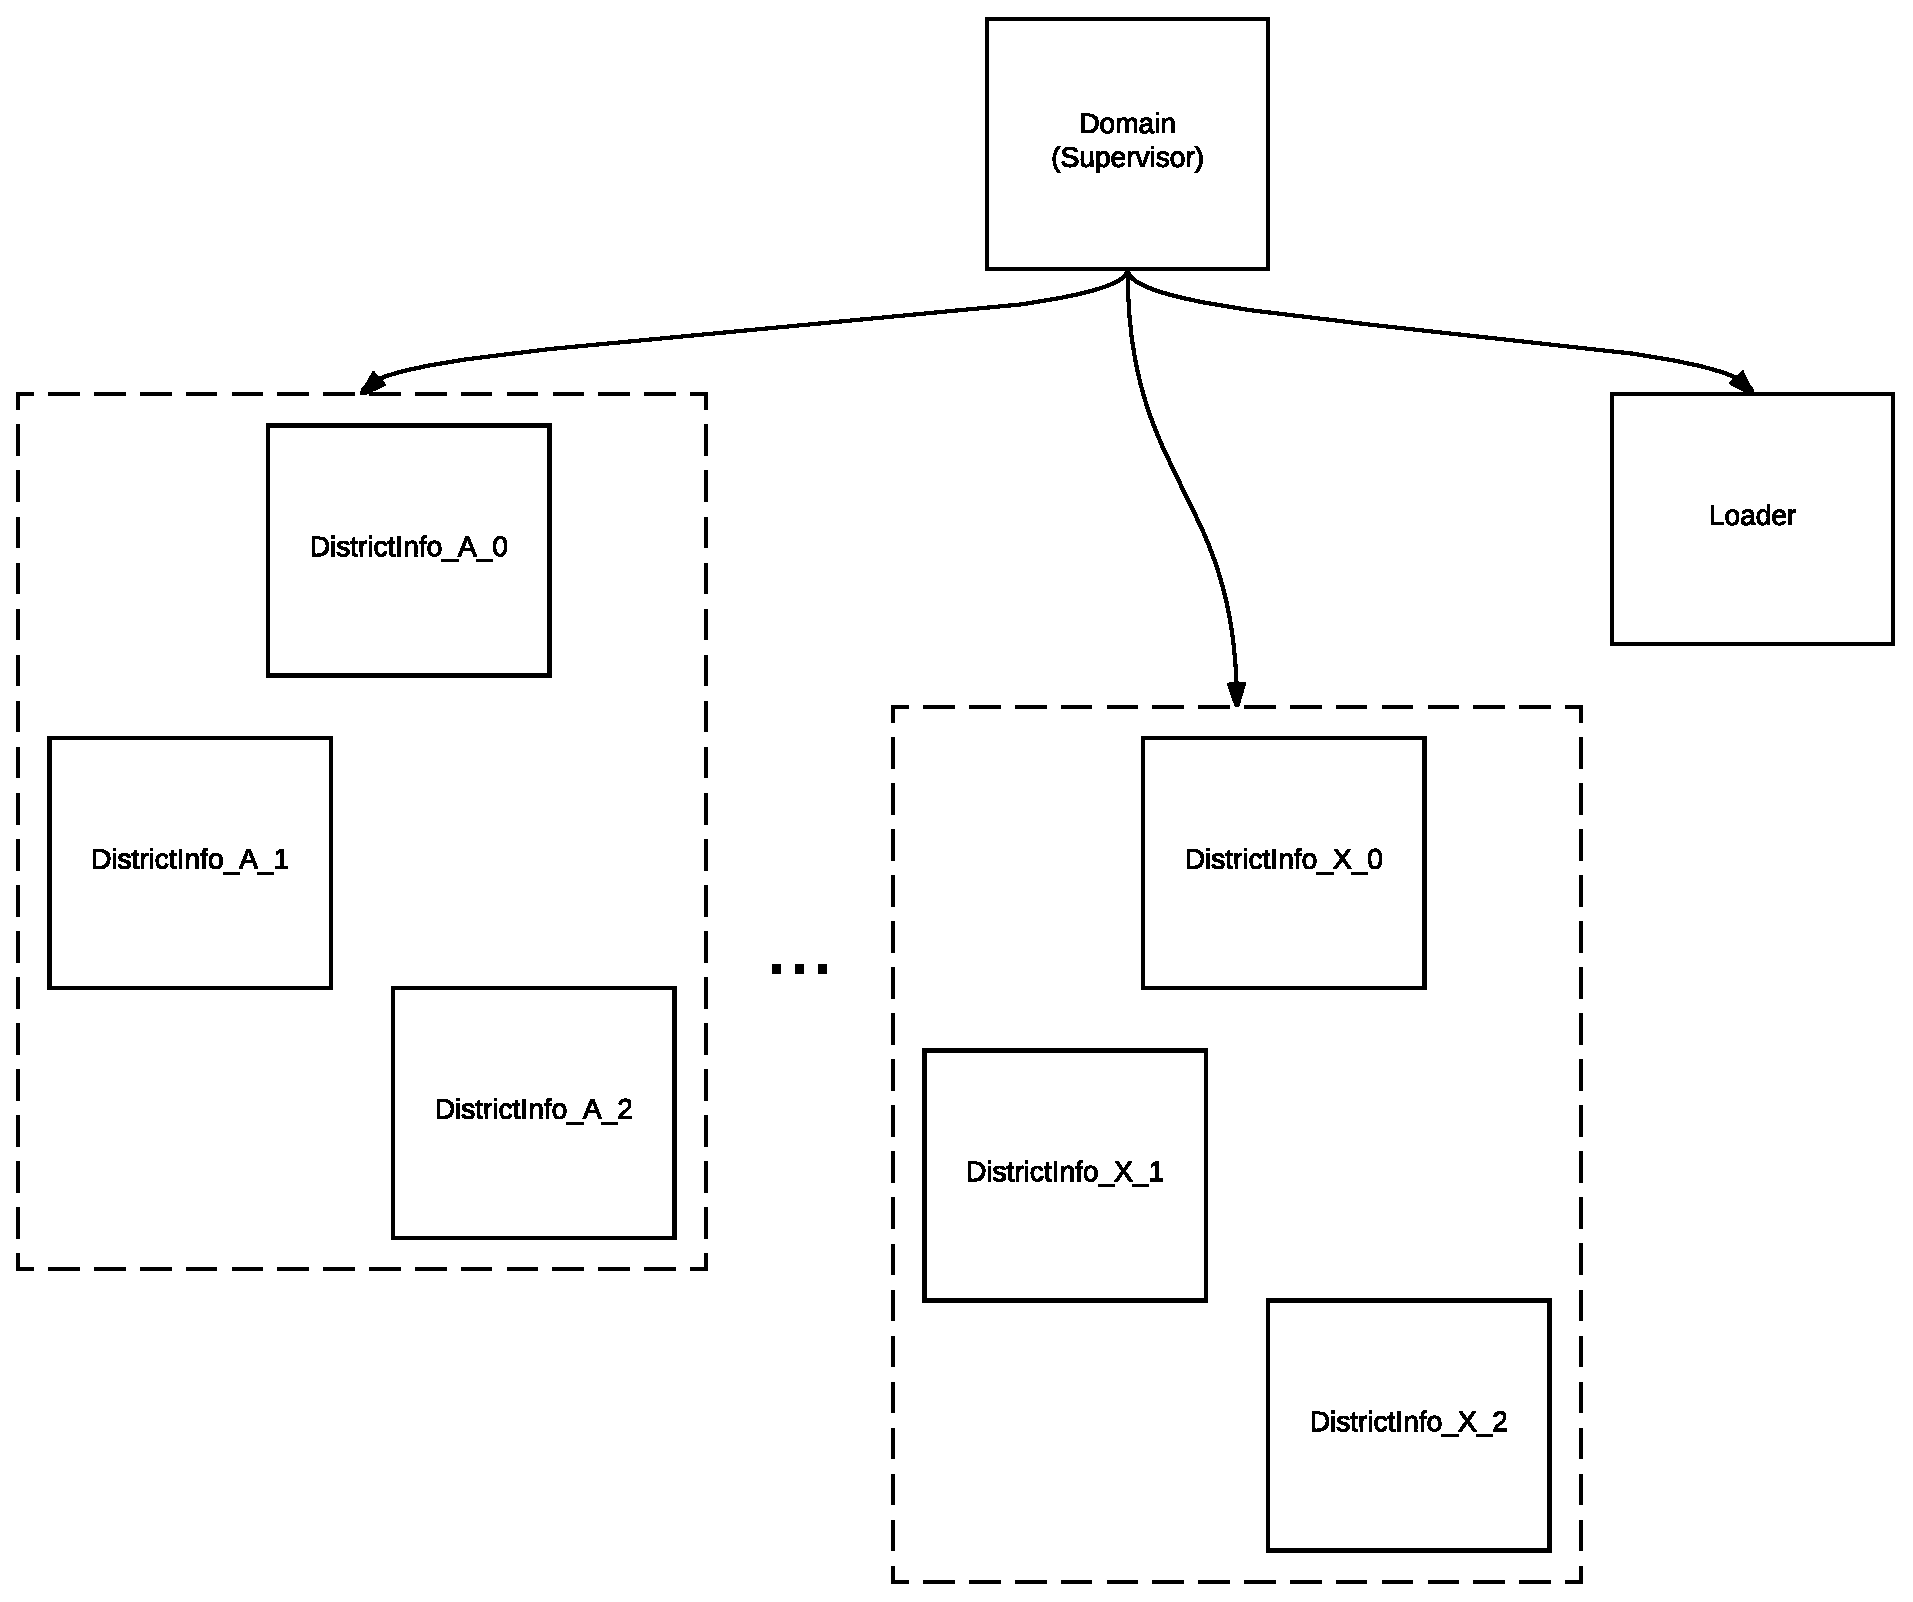
\includegraphics[width=.95\columnwidth]{images/implementation/as-domain.eps}
  \caption{Domain supervision tree}
  \label{fig:impl-as-domain}
\end{figure}

\subsubsection{Interface}

We will focus on some key components of the \texttt{Interface} sub-system
implementation.

\paragraph{PubSub}
\texttt{DistrictChannel} is an
implementation we provided for the \texttt{Channel} behavior. As we can see
in Figure \ref{fig:impl-as-pubsub}, \texttt{UserSocket}s subscribe to the
Phoenix pub/sub system for the city simulator.
Sockets reach \texttt{DistrictChannel} through an \texttt{Endpoint}.
Each socket is always subscribed to a district, and could be additionally
subscribed to a traveler. Therefore:

\begin{itemize}
  \item when a user requires to join the \texttt{DistrictChannel}, it will
    be immediately subscribed to the district she is interested in;
  \item later on, the user may request to have updates on a specific traveler
    by making a subscription to a specific traveler topic.
\end{itemize}

Finally, in \texttt{DistrictChannel} we filter (and eventually process)
outgoing information by implementing specific \texttt{handle\_out} callbacks.
Thanks to this, we are able to avoid unnecessary traffic towards the clients.

\paragraph{Input pipeline}
Events and updates arrive at the application server starting from an
\texttt{InputStream}. This process is a Wabbit GenStage which
basically receives messages from a RabbitMQ topic exchange and forwards them
to a \texttt{Formatter}.
A \texttt{Formatter} is a process which just extracts basic information from
the incoming messages and transform them in a format used by the application
server processes.
Then, messages are piped through an \texttt{InternalDispatcher} process, which
can eventually dispatch some information to some processes in the Application
Server; for example, it sends updates to district trackers when a traveler
moves from a district to another one.
Finally, messages are broadcasted to \texttt{Interface.Endpoint} by
providing the payload and the topic of the message.

\paragraph{Output}
The Application Server is also able to send minimal control information (start
messages) to the cities used for simulations. This is done via a process called
\texttt{OutputStream}\footnote{actually, this process is replicated once for
each city}, which dispatches control messages to the right backend node.

\begin{figure}[H]
  \centering
  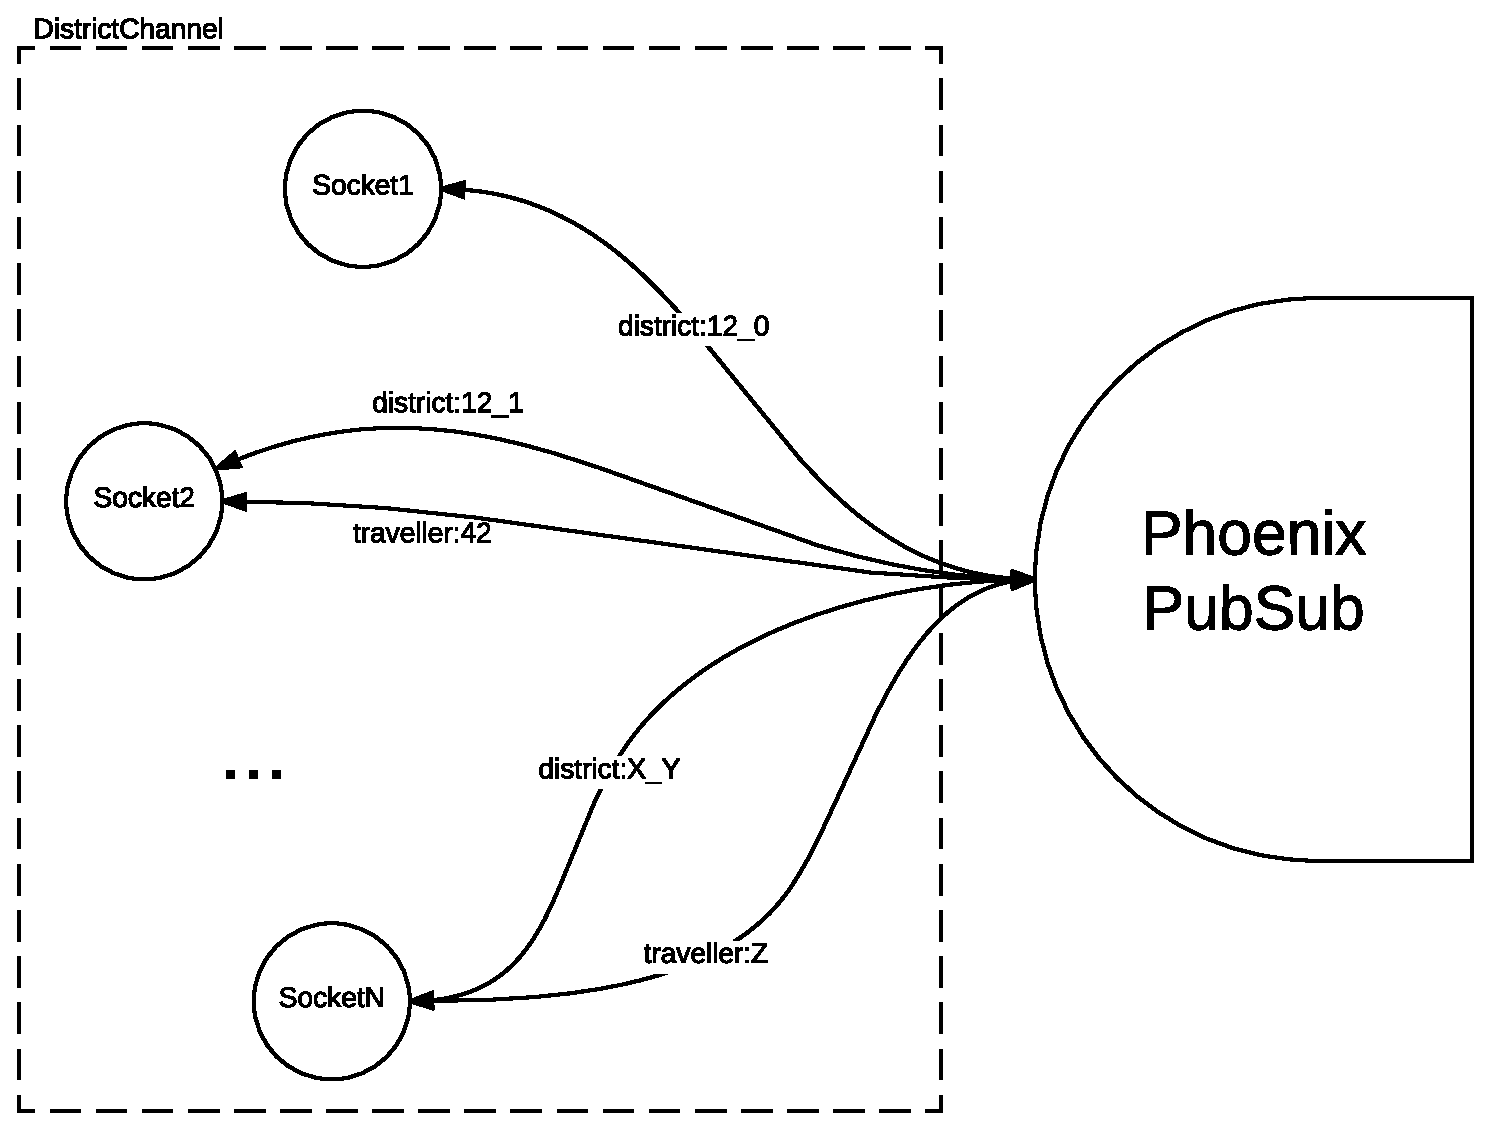
\includegraphics[width=1.1\columnwidth]{images/implementation/as-chan-pubsub.eps}
  \caption{Application Server architecture}
  \label{fig:impl-as-pubsub}
\end{figure}
